
%%%%%%%%%%%%%%%%%%%%%%%%%%%%%%%%%%%%%%%%%%%%%%%%%%%%%%%%
%
% Copyright (c) 2003-2008 by University of Queensland
% Earth Systems Science Computational Center (ESSCC)
% http://www.uq.edu.au/esscc
%
% Primary Business: Queensland, Australia
% Licensed under the Open Software License version 3.0
% http://www.opensource.org/licenses/osl-3.0.php
%
%%%%%%%%%%%%%%%%%%%%%%%%%%%%%%%%%%%%%%%%%%%%%%%%%%%%%%%%


\section{The First Steps}
\label{FirstSteps} 

\begin{figure}
\centerline{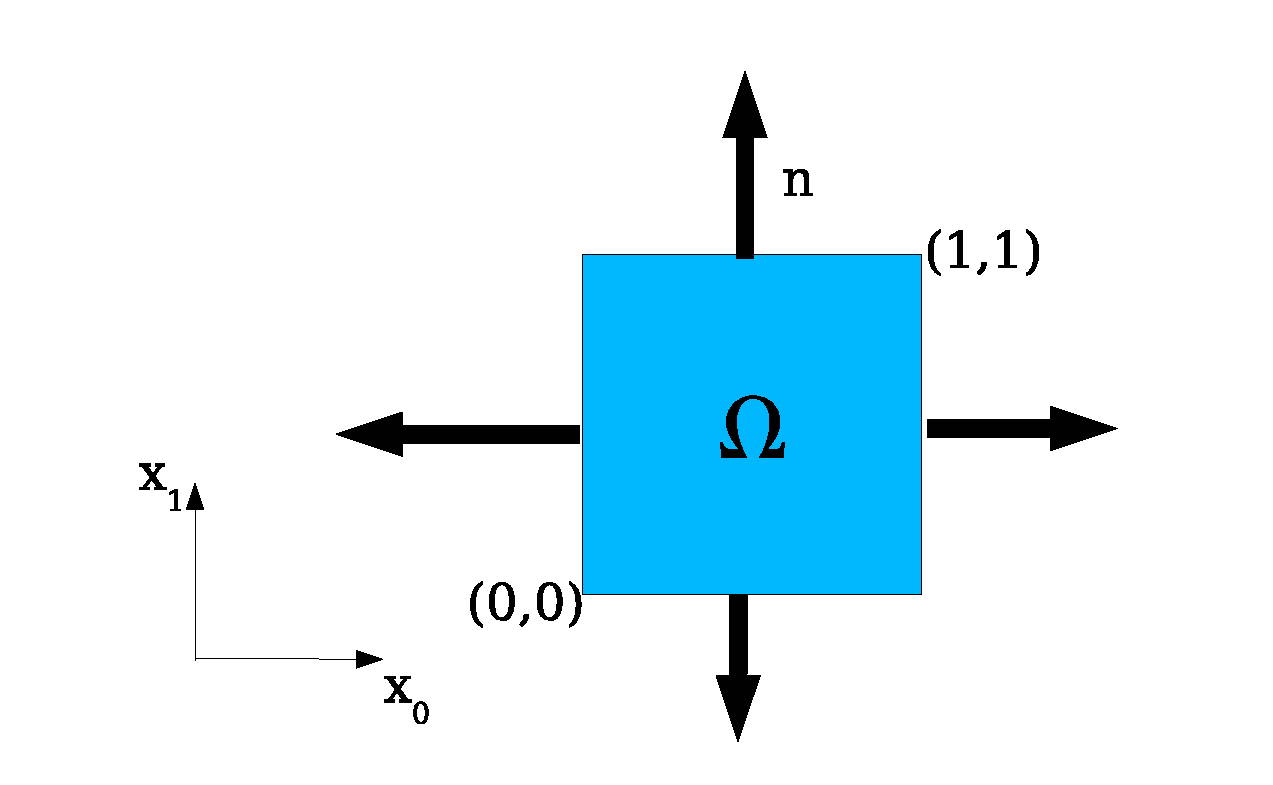
\includegraphics[width=\figwidth]{figures/FirstStepDomain}}
\caption{Domain $\Omega=[0,1]^2$ with outer normal field $n$.}
\label{fig:FirstSteps.1}
\end{figure}

In this chapter we give an introduction how to use \escript to solve 
a partial differential equation \index{partial differential equation} (PDE \index{partial differential equation!PDE}). We assume you are at least a little familiar with Python. The knowledge presented at the Python tutorial at \url{http://docs.python.org/tut/tut.html}
is more than sufficient.

The PDE \index{partial differential equation} we wish to solve is the Poisson equation \index{Poisson equation} 
\begin{equation}
-\Delta u =f 
\label{eq:FirstSteps.1}
\end{equation}
for the solution $u$. The function $f$ is the given right hand side. The domain of interest, denoted by $\Omega$,
is the unit square 
\begin{equation}
\Omega=[0,1]^2=\{ (x\hackscore 0;x\hackscore 1) | 0\le x\hackscore{0} \le 1 \mbox{ and } 0\le x\hackscore{1} \le 1 \}
\label{eq:FirstSteps.1b}
\end{equation}
The domain is shown in \fig{fig:FirstSteps.1}.

$\Delta$ denotes the Laplace operator\index{Laplace operator}, which is defined by
\begin{equation}
\Delta u = (u\hackscore {,0})\hackscore{,0}+(u\hackscore{,1})\hackscore{,1}
\label{eq:FirstSteps.1.1}
\end{equation}
where, for any function $u$ and any direction $i$, $u\hackscore{,i}$
denotes the partial derivative \index{partial derivative} of $u$ with respect to $i$.  
\footnote{You
may be more familiar with the Laplace operator\index{Laplace operator} being written
as $\nabla^2$, and written in the form
\begin{equation*}
\nabla^2 u = \nabla^t \cdot \nabla u =  \frac{\partial^2 u}{\partial x\hackscore 0^2} 
+ \frac{\partial^2 u}{\partial  x\hackscore 1^2}
\end{equation*}
and \eqn{eq:FirstSteps.1} as
\begin{equation*}
-\nabla^2 u = f
\end{equation*}
}
Basically, in the subindex of a function, any index to the left of the comma denotes a spatial derivative with respect 
to the index. To get a more compact form we will write $w\hackscore{,ij}=(w\hackscore {,i})\hackscore{,j}$
which leads to
\begin{equation}
\Delta u = u\hackscore{,00}+u\hackscore{,11}=\sum\hackscore{i=0}^2 u\hackscore{,ii}
\label{eq:FirstSteps.1.1b}
\end{equation}
We often find that use
of nested $\sum$ symbols makes formulas cumbersome, and we use the more
convenient Einstein summation convention \index{summation convention}. This 
drops the $\sum$ sign and assumes that a summation is performed over any repeated index.
For instance we write
\begin{eqnarray}
x\hackscore{i}y\hackscore{i}=\sum\hackscore{i=0}^2 x\hackscore{i}y\hackscore{i}   \\
x\hackscore{i}u\hackscore{,i}=\sum\hackscore{i=0}^2 x\hackscore{i}u\hackscore{,i}   \\
u\hackscore{,ii}=\sum\hackscore{i=0}^2 u\hackscore{,ii} \\
x\hackscore{ij}u\hackscore{i,j}=\sum\hackscore{j=0}^2\sum\hackscore{i=0}^2 x\hackscore{ij}u\hackscore{i,j}   \\
\label{eq:FirstSteps.1.1c}
\end{eqnarray}
With the summation convention we can write the Poisson equation \index{Poisson equation} as
\begin{equation}
- u\hackscore{,ii} =1 
\label{eq:FirstSteps.1.sum}
\end{equation}
where $f=1$ in this example.

On the boundary of the domain $\Omega$ the normal derivative $n\hackscore{i} u\hackscore{,i}$
of the solution $u$ shall be zero, ie. $u$ shall fulfill
the homogeneous Neumann boundary condition\index{Neumann
boundary condition!homogeneous}
\begin{equation}
n\hackscore{i} u\hackscore{,i}= 0 \;.
\label{eq:FirstSteps.2}
\end{equation}
$n=(n\hackscore{i})$ denotes the outer normal field
of the domain, see \fig{fig:FirstSteps.1}. Remember that we 
are applying the Einstein summation convention \index{summation convention}, i.e
$n\hackscore{i} u\hackscore{,i}= n\hackscore{0} u\hackscore{,0} +
n\hackscore{1} u\hackscore{,1}$. 
\footnote{Some readers may familiar with the notation
\begin{equation*}
\frac{\partial u}{\partial n} = n\hackscore{i} u\hackscore{,i}
\end{equation*}
for the normal derivative.}
The Neumann boundary condition of \eqn{eq:FirstSteps.2} should be fulfilled on the
set $\Gamma^N$ which is the top and right edge of the domain:
\begin{equation}
\Gamma^N=\{(x\hackscore 0;x\hackscore 1) \in \Omega | x\hackscore{0}=1 \mbox{ or } x\hackscore{1}=1  \}
\label{eq:FirstSteps.2b}
\end{equation}
On the bottom and the left edge of the domain which is defined
as 
\begin{equation}
\Gamma^D=\{(x\hackscore 0;x\hackscore 1) \in \Omega | x\hackscore{0}=0 \mbox{ or } x\hackscore{1}=0  \}
\label{eq:FirstSteps.2c}
\end{equation}
the solution shall be identically zero:
\begin{equation}
u=0 \; .
\label{eq:FirstSteps.2d}
\end{equation}
This kind of boundary condition is called a homogeneous Dirichlet boundary condition
\index{Dirichlet boundary condition!homogeneous}. The partial differential equation in \eqn{eq:FirstSteps.1.sum} together
with the Neumann boundary condition \eqn{eq:FirstSteps.2} and 
Dirichlet boundary condition in \eqn{eq:FirstSteps.2d} form a so
called boundary value
problem\index{boundary value problem} (BVP\index{boundary value problem!BVP}) for 
the unknown
function $u$. 


\begin{figure}
\centerline{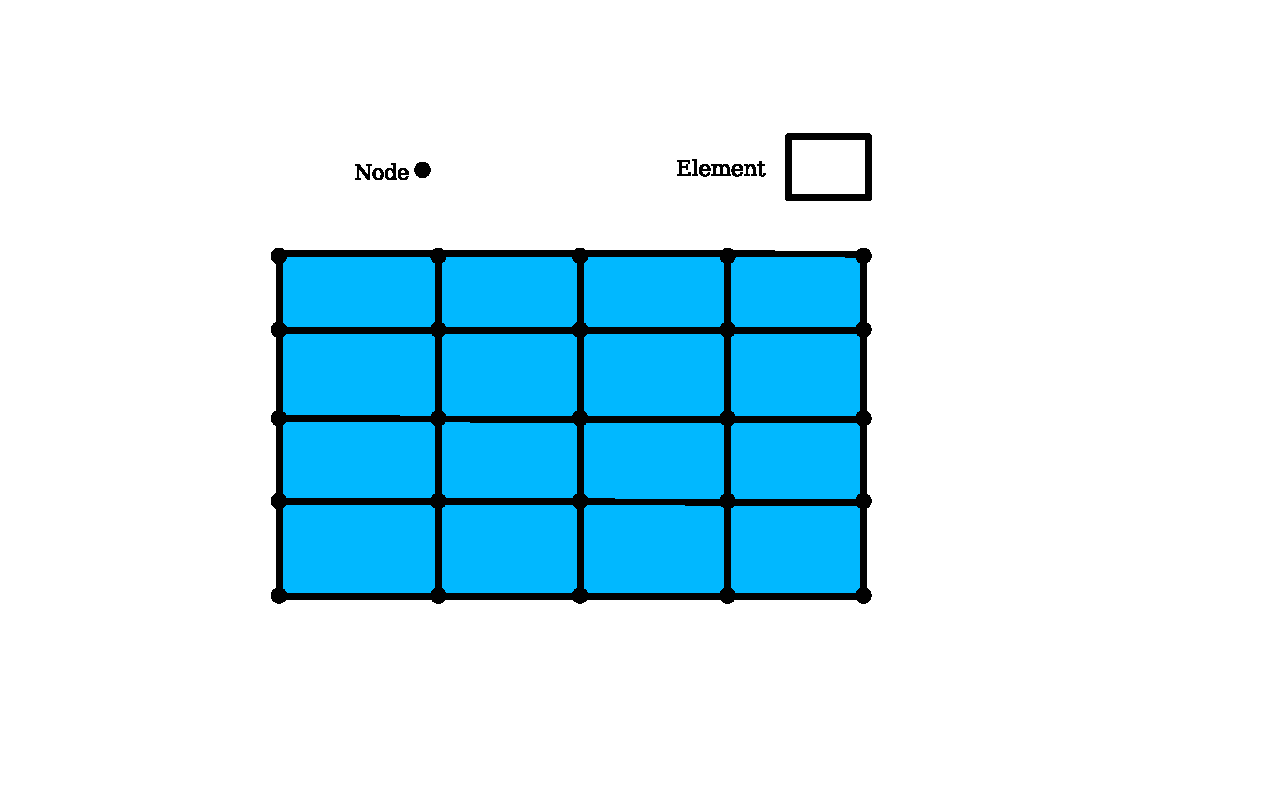
\includegraphics[width=\figwidth]{figures/FirstStepMesh.eps}}
\caption{Mesh of $4 \time 4$ elements on a rectangular domain.  Here
each element is a quadrilateral and described by four nodes, namely
the corner points. The solution is interpolated by a bi-linear
polynomial.}
\label{fig:FirstSteps.2}
\end{figure}

In general the BVP\index{boundary value problem!BVP} cannot be solved analytically and numerical
methods have to be used construct an approximation of the solution
$u$. Here we will use the finite element method\index{finite element
method} (FEM\index{finite element
method!FEM}). The basic idea is to fill the domain with a
set of points called nodes. The solution is approximated by its
values on the nodes\index{finite element
method!nodes}. Moreover, the domain is subdivided into smaller
sub-domains called elements \index{finite element
method!element}. On each element the solution is
represented by a polynomial of a certain degree through its values at
the nodes located in the element. The nodes and its connection through
elements is called a mesh\index{finite element
method!mesh}. \fig{fig:FirstSteps.2} shows an
example of a FEM mesh with four elements in the $x_0$ and four elements
in the $x_1$ direction over the unit square.  
For more details we refer the reader to the literature, for instance
\Ref{Zienc,NumHand}.

\escript provides the class \Poisson to define a Poisson equation \index{Poisson equation}.
(We will discuss a more general form of a PDE \index{partial differential equation!PDE} 
that can be defined through the \LinearPDE class later). The instantiation of
a \Poisson class object requires the specification of the domain $\Omega$. In \escript
the \Domain class objects are used to describe the geometry of a domain but it also
contains information about the discretization methods and the actual solver which is used
to solve the PDE. Here we are using the FEM library \finley \index{finite element
method}. The following statements create the \Domain object \var{mydomain} from the 
\finley method \method{Rectangle}
\begin{python}
  from esys.finley import Rectangle
  mydomain = Rectangle(l0=1.,l1=1.,n0=40, n1=20)
\end{python}
In this case the domain is a rectangle with the lower, left corner at point $(0,0)$ and
the right, upper corner at $(\var{l0},\var{l1})=(1,1)$.
The arguments \var{n0} and \var{n1} define the number of elements in $x\hackscore{0}$ and
$x\hackscore{1}$-direction respectively. For more details on \method{Rectangle} and
other \Domain generators within the \finley module,
see \Chap{CHAPTER ON FINLEY}.

The following statements define the \Poisson class object \var{mypde} with domain \var{mydomain} and
the right hand side $f$ of the PDE to constant $1$: 
\begin{python}
  from esys.escript.linearPDEs import Poisson
  mypde = Poisson(mydomain)
  mypde.setValue(f=1)
\end{python}
We have not specified any boundary condition but the 
\Poisson class implicitly assumes homogeneous Neuman boundary conditions \index{Neumann
boundary condition!homogeneous} defined by \eqn{eq:FirstSteps.2}. With this boundary 
condition the BVP\index{boundary value problem!BVP} we have defined has no unique solution. In fact, with any solution $u$
and any constant $C$ the function $u+C$ becomes a solution as well. We have to add 
a Dirichlet boundary condition \index{Dirichlet boundary condition}. This is done 
by defining a characteristic function \index{characteristic function} 
which has positive values at locations $x=(x\hackscore{0},x\hackscore{1})$ where Dirichlet boundary condition is set
and $0$ elsewhere. In our case of $\Gamma^D$ defined by \eqn{eq:FirstSteps.2c},
we need to construct a function \var{gammaD} which is positive for the cases $x\hackscore{0}=0$ or $x\hackscore{1}=0$. To get 
an object \var{x} which contains the coordinates of the nodes in the domain use
\begin{python}
  x=mydomain.getX() 
\end{python}
The method \method{getX} of the \Domain \var{mydomain} 
gives access to locations 
in the domain defined by \var{mydomain}. The object \var{x} is actually a \Data object which will be
discussed in \Chap{ESCRIPT CHAP} in more detail. What we need to know here is that 

\var{x} has \Rank (number of dimensions) and a \Shape (list of dimensions) which can be viewed by 
calling the \method{getRank} and \method{getShape} methods:
\begin{python}
  print "rank ",x.getRank(),", shape ",x.getShape()
\end{python}
This will print something like
\begin{python}
  rank 1, shape (2,)
\end{python}
The \Data object also maintains type information which is represented by the 
\FunctionSpace of the object. For instance
\begin{python}
  print x.getFunctionSpace()
\end{python}
will print 
\begin{python}
  Function space type: Finley_Nodes on FinleyMesh 
\end{python}
which tells us that the coordinates are stored on the nodes of (rather than on points in the interior of) a \finley mesh.
To get the  $x\hackscore{0}$ coordinates of the locations we use the
statement 
\begin{python}
  x0=x[0]
\end{python}
Object \var{x0} 
is again a \Data object now with \Rank $0$ and 
\Shape $()$. It inherits the \FunctionSpace from \var{x}:
\begin{python}
  print x0.getRank(),x0.getShape(),x0.getFunctionSpace()
\end{python}
will print
\begin{python}
  0 () Function space type: Finley_Nodes on FinleyMesh 
\end{python}
We can now construct a function \var{gammaD} which is only non-zero on the bottom and left edges
of the domain with
\begin{python}
  from esys.escript import whereZero
  gammaD=whereZero(x[0])+whereZero(x[1])
\end{python}

\code{whereZero(x[0])} creates function which equals $1$ where \code{x[0]} is (almost) equal to zero 
and $0$ elsewhere. 
Similarly, \code{whereZero(x[1])} creates function which equals $1$ where \code{x[1]} is 
equal to zero and $0$ elsewhere.
The sum of the results of \code{whereZero(x[0])} and \code{whereZero(x[1])} 
gives a function on the domain \var{mydomain} which is exactly positive where $x\hackscore{0}$ or $x\hackscore{1}$ is equal to zero.
Note that \var{gammaD} has the same \Rank, \Shape and \FunctionSpace like \var{x0} used to define it. So from 
\begin{python}
  print gammaD.getRank(),gammaD.getShape(),gammaD.getFunctionSpace()
\end{python}
one gets 
\begin{python}
  0 () Function space type: Finley_Nodes on FinleyMesh 
\end{python}
An additional parameter \var{q} of the \code{setValue} method of the \Poisson class defines the 
characteristic function \index{characteristic function} of the locations
of the domain where homogeneous Dirichlet boundary condition \index{Dirichlet boundary condition!homogeneous}
are set. The complete definition of our example is now: 
\begin{python}
  from esys.linearPDEs import Poisson
  x = mydomain.getX()
  gammaD = whereZero(x[0])+whereZero(x[1])
  mypde = Poisson(domain=mydomain)
  mypde.setValue(f=1,q=gammaD)
\end{python}
The first statement imports the \Poisson class definition from the \linearPDEs module \escript package.
To get the solution of the Poisson equation defined by \var{mypde} we just have to call its
\method{getSolution}. 

Now we can write the script to solve our Poisson problem
\begin{python}
  from esys.escript import *
  from esys.escript.linearPDEs import Poisson
  from esys.finley import Rectangle
  # generate domain:
  mydomain = Rectangle(l0=1.,l1=1.,n0=40, n1=20)
  # define characteristic function of Gamma^D
  x = mydomain.getX()
  gammaD = whereZero(x[0])+whereZero(x[1])
  # define PDE and get its solution u
  mypde = Poisson(domain=mydomain)
  mypde.setValue(f=1,q=gammaD)
  u = mypde.getSolution()
  # write u to an external file
  saveVTK("u.xml",sol=u)
\end{python}
The entire code is available as \file{poisson.py} in the \ExampleDirectory

The last statement writes the solution (tagged with the name "sol") to a file named \file{u.xml} in 
\VTK file format.
Now you may run the script and visualize the solution using \mayavi:
\begin{verbatim}
  python poisson.py
  mayavi -d u.xml -m SurfaceMap
\end{verbatim}
See \fig{fig:FirstSteps.3}.

\begin{figure}
\centerline{\includegraphics[width=\figwidth]{figures/FirstStepResult.eps}}
\caption{Visualization of the Poisson Equation Solution for $f=1$}
\label{fig:FirstSteps.3}
\end{figure}

